% Be sure to write chapter titles in ALL CAPS
\chapter{\uppercase{BACKGROUND}}

This chapter is divided into four sections.  First, I provide some background on JavaScript and the characteristics of the language that make it challenging to test.  Second, I explain a traditional URL format, describing the relative ease of programmatically discovering variables.  Third, I explain the more recent semantic URL format and some of the difficulties introduced with systemic variable identification.  Fourth, I introduce and describe an algorithm for statistically analyzing an application's URL structure to identify variables.

\section{JavaScript Background}
Due to its distribution in all browsers, JavaScript is the primary language for Rich Web Applications (RWA).  It plays a central role in RWAs by updating styles and modifying application structure markup (i.e., the Document Object Model or DOM).  It also is the key data transport mechanism for interacting with the server via it's XmlHttpRequest (XHR) object.  As a language, it is dynamic, weakly typed, interpreted, and prototype-based.  With it's features such as first-class functions, it supports multiple development paradigms, including: object-oriented, imperative, and functional.  JavaScript can either be loaded by the browser as static code or it can be dynamically created at runtime using an ``eval( )'' function.  

Two traits make JavaScript particularly vulnerable to faults.  First, as a dynamically typed, interpreted language it does not benefit as much as strongly typed, compiled languages from static code analysis.  Lint-like tools exist for JavaScript but they typically focus on syntax.  Second, JavaScript is designed to respond to timers and browser events such as clicks, hovering, or key presses.  This makes it difficult to test event driven code in a development environment as it requires simulating those events to test.

New JavaScript frameworks such as Backbone.js have helped with the consistency of JavaScript code being developed.  They have helped isolate faults to mostly appearance related exceptions.  In the next chapter, I describe in detail the types of web application and JavaScript faults in the context of a sample application and how those faults are identified with the developed testing strategies.

\section{Traditional URL Formats}
Rich web applications, along with a migration from server-side to client-side JavaScript based frameworks, have generally adopted a different URL structure from the traditional format defined in RFC 1738\cite{berners1994uniform}.  A traditional URL structure defined in the RFC 1738 standard, follows the format:

\begin{figure}[h]
\centering
http://\textless host\textgreater :\textless port\textgreater /\textless path\textgreater ?\textless searchpart\textgreater
\end{figure}

The \textless searchpart\textgreater\ of a traditional URL format is composed of a series of key-value pairs that start after the question mark.  Keys and values are separated by an equals sign and the key-value pairs are separated by an ampersand. An example of a \textless searchpart\textgreater, more frequently called a query string, following the question mark of a URL is as follows:

\begin{figure}[h]
\centering
key1=value1\&key2=value2
\end{figure}

Traditional URL structures, as defined in RFC 1738, with their key-value pairs are very easy to programmatically identify and parse.  This well structured format allows a testing solution to quickly determine variable names and values for combinatorial testing.

\section{Semantic URL Formats}
Rich web applications have departed from this traditional \textless searchpart\textgreater\ format in favor of a more user friendly, more permanent format\cite{tbl2008}.  This new format is often referred to as semantic or clean URLs.  One goal of semantic URLs is to provide an immediate, human understandable format of resources.  Instead of clearly identifying variables and their values as key-value pairs after a question mark in the \textless searchpart\textgreater\ section of a URL, rich web applications typically combine their variables and values as part of the \textless path\textgreater\ portion of the URL.  While easier for a human to understand, this structure makes it difficult to programmatically discover variables for combinatorial testing.

As an example of a semantic URL, imagine a rich web application that provides census information on states, counties, and cities over a certain population of the United States.  A semantic URL for this application might look as follows:
\begin{figure}[h]
\centering
  http://example.com/\#/state/utah/county/cache/city/logan
\end{figure}

This example is a well structured semantic URL.  Each variable is preceded by a descriptive key (e.g., ``state'' precedes ``ut'' and ``county'' precedes ``cache'').  Unfortunately, no standards exist for semantic URL structures, and many rich web applications do not always find it practical to follow this industry best practice of associated keys and values for variables.  This application could have just as easily been developed with a URL structure:

\begin{figure}[h]
\centering
  http://example.com/\#/utah/cache/logan
\end{figure}

Due to the variety of formats used in semantic URLs and the absence of an industry standard, identifying variables for combinatorial testing can be difficult.  In the next section I propose an algorithm for variable identification regardless of the example structures shown above.

\section{Variable Detection Algorithm for Semantic URLs}
In order to address the complexities of identifying variables in semantic URLs, I propose the following algorithm that processes all URLs from a rich web application and identifies the location of variables in a URL structure.

The algorithm processes each URL of the rich web application and then subsequently processes each portion of the URL \textless path\textgreater.  It then combines them into a common hierarchical graph to allow analysis of the application structure.  The key to identifying the location of variables is by calculating branching complexity as each URL is processed.  This branching complexity is measured by creating a graph node at each URL \textless path\textgreater\ portion (e.g., each part of the URL path separated by a ``/'' character).  As each node is created, the Strahler number is calculated by looking at all the previous child nodes\cite{gleyzer2004fast}.  Identifying the degree of branching at each level of the URL path allows for analysis of the branching complexity for each abstract portion of the URLS of the application.

The algorithm is listed in Figure~\ref{algorithm} followed in the next section by a detailed description.

\begin{figure}
\begin{lstlisting}
	foreach(url in urls) {
		Node previousNode = retrieveOrCreateNode(url);
		int position = url.length();
		String shortenedUrl;
		while(position > fragmentIdentifier) {
			position = url.lastIndexOf("/");
			if(position > 0) {
				shortenedUrl = url.substring(0, position);
				Node node = retrieveOrCreateNode(shortenedUrl);
				int branchingComplexity = calculateBranchingComplexity(node);
				node.setProperty(BRANCHING_COMPLEXITY, branchingComplexity);
				previousNode.createRelationshipTo(node, 
						RelationshipTypes.CHILD_OF);		
				previousNode = node;
			}
			else {
				break;
			}
		}
		Node last = retrieveOrCreateNode(shortenedUrl);
	}
\end{lstlisting}
\caption{Algorithm for variable identification of semantic URLs}
\label{algorithm}
\end{figure}

\section{Algorithm Description}
For brevity, the algorithm, as listed, assumes the possession of a list every possible URL available in the application.  The sample rich web application discussed in this section has approximately 200,000 different semantic URLs.  A better implementation of the algorithm would be to crawl the site in a depth-first, non-deterministic fashion recording and processing each URL (i.e., applying this algorithm in-line as the site is crawled).

The algorithm proceeds to lob off each outer part of the URL path until the position variable listed on line 103 is less than the fragment identifier character position in the URL.

Starting with the example URL listed previously, the algorithm values are processed in the following list.

\begin{enumerate}
	\item http://example.com/\#/state/ut/county/cache/city/logan.
	\item http://example.com/\#/state/ut/county/cache/city
	\item http://example.com/\#/state/ut/county/cache
	\item http://example.com/\#/state/ut/county
	\item http://example.com/\#/state/ut/
	\item http://example.com/\#/state
	\item http://example.com/\#
\end{enumerate}

As we're focused on the \textless path\textgreater\ portion of the URL, the algorithm stops processing when the position index of the last instance of the path separator ``/'' is less than the position index of the fragment identifier (the ``\#'' character).  Continuing on line 108, the algorithm then either retrieves (if it already exists) or creates (if the remaining URL has not been processed) a new node that represents that portion of the URL.  The algorithm works its way backwards from full URL to just the host to allow for the easy calculation of the Strahler number used to identify branching complexity in line 109.  On line 111 the algorithm creates the edge between the current and the previous node.  It then assigns the current node to the previous node so it can continue processing if needed.

An additional benefit of having the application structure in a common graph is it makes it easy to visually identify branching complexity as in Figure~\ref{fig:visualization}.  Dark areas represent extensive branching that is associated with variables in semantic URLs.

\begin{figure}[htb]
\centering
%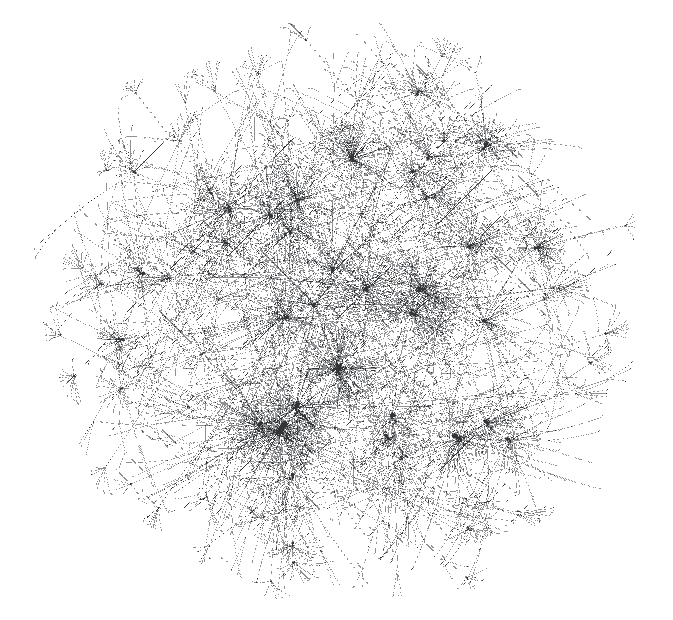
\includegraphics[width=0.9\textwidth]{images/thesis-graph-figure.png}
\caption{A visual representation of branching complexity in an application structure.}
\label{fig:visualization}
\end{figure}